\section{Reconstruction for VLA Observations}

Compressed Sensing Reconstruction used on two different tasks:
\begin{itemize}
	\item Center detection on sunburst data
	\item Reconstruction from incomplete measurements of Supernova Remnant G55
\end{itemize}

Two different problems. One is the 

Structure potentially smaller than the primary beam.



\subsection{Sunburst Center Detection}

Sub- Primary Beam.
CS Objective Function

Figure: Dirty Map Peak, CLEAN, Single Peak Clean, Single Peak CS Reconstruction

\begin{figure}
	
\end{figure}

Wider Variance


\subsection{Reconstruction of Supernova Remnant G55}
\begin{figure}[h]
	\centering
	\begin{subfigure}[b]{0.45\linewidth}
		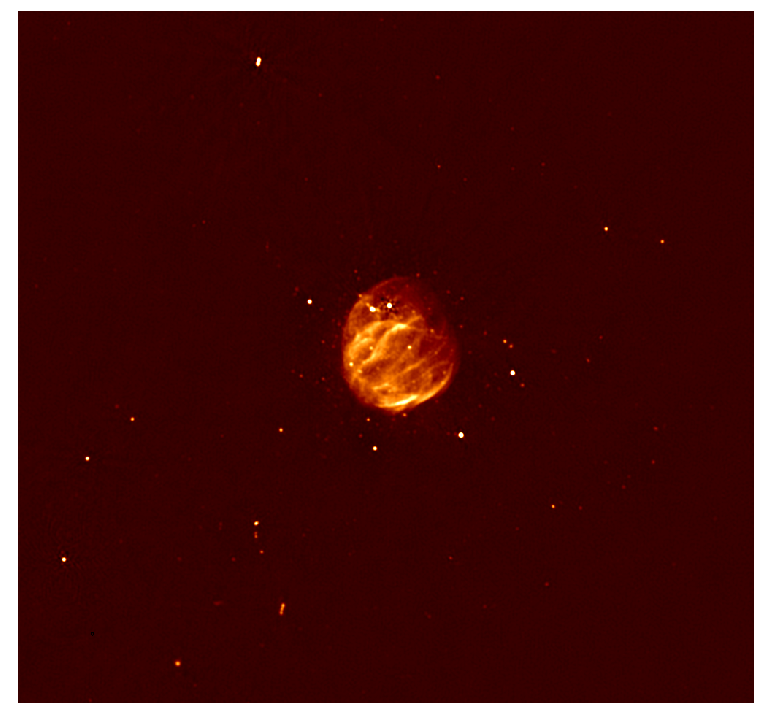
\includegraphics[width=\linewidth, trim={230px 210px 225px 200px}, clip]{./chapters/05.results/pic_G55_7.png}
		\caption{Reconstruction by NRAO.  Source:\cite{nraoG55}}
		\label{results:g55:nrao:rec}
	\end{subfigure}
	\begin{subfigure}[b]{0.45\linewidth}
		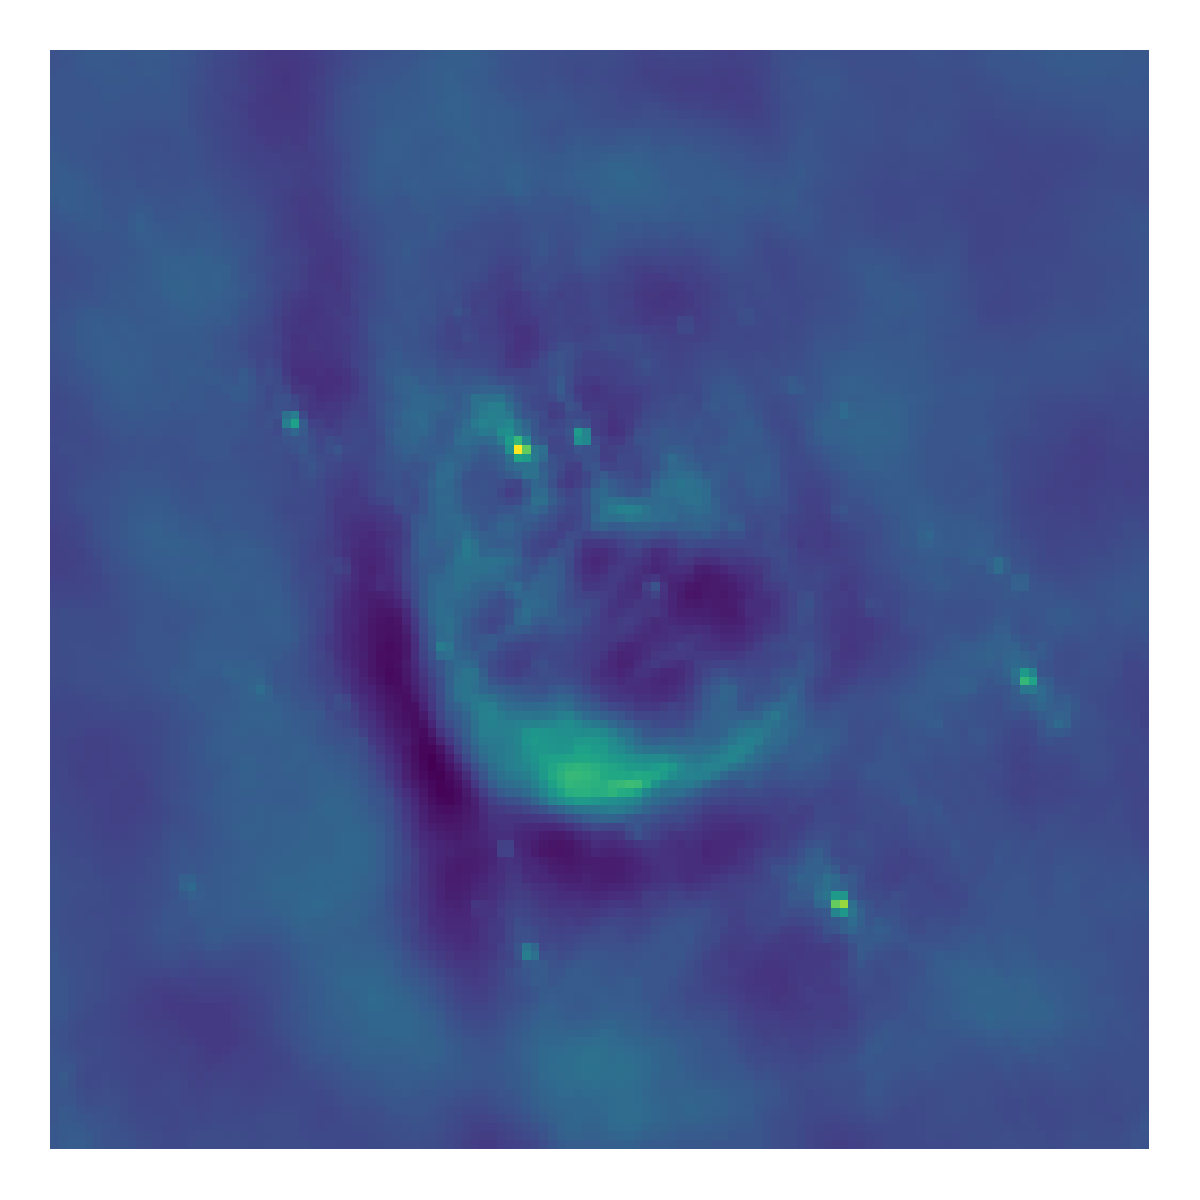
\includegraphics[width=\linewidth, trim={18px 19px 18px 18px}, clip]{./chapters/05.results/g55/raw_image.png}
		\caption{Dirty Image}
		\label{results:g55:nrao:dirty}
	\end{subfigure}
	\caption{SNR G55 source observed by VLA.}
	\label{results:g55:nrao}
\end{figure}

The supernova remnant (SNR) G55 was observed by VLA. 10 seconds of the 8 hour observation is publicly available through the CASA imaging tutorial\cite{casaImagingGuide}. \ref{results:g55:nrao:dirty} is the dirty image calculated from the 10 second observation. The full 8 hours are not readily available. The image \ref{results:g55:nrao:rec} is a reconstruction from an unknown VLA observation. The deconvolution algorithm is also unknown. For this project, the reconstructed image is assumed to show the true image of the sky.

\ref{results:g55:nrao} shows G55 to be a slightly "egg shaped" extended emission with six strong point sources. Several fainter point sources are inside and around the egg shaped extended emission. The dirty image \ref{results:g55:nrao:dirty} shows a corrupted version of G55. The six strong point sources are clearly visible as are the brighter parts of the extended emission. The dirty image also shows a negative "trench" striking through the image as well as brighter regions around the remnant. 

The size of the images \ref{results:g55:nrao} is about twice the size of the primary beam (the primary beam is approximately the size of the extended emission). In the real world, wide field imaging would be used. In this project, small field of view imaging was used because it is quicker to compute. 
It limits the dynamic range of the dirty image, the whole task gets harder. 

The CLEAN algorithm gets compared to Compressed Sensing Reconstructions. The parameters of CLEAN were taken from the CASA imaging tutorial\cite{casaImagingGuide}. The reconstructed images of Compressed Sensing are constrained to have no negative pixels. Negative pixels are not physically plausible and was shown to improve Compressed Sensing reconstructions for synthetic data\cite{mcewen2011compressed}. In total six different priors were tested with the analysis objective:
\begin{enumerate}
	\item No Regularization
	\item L1
	\item L2
	\item L1+L2
	\item Total Variation
	\item Starlet Transform
\end{enumerate}

The regularization parameter $\lambda$ needs to be estimated for each prior. The Miller\cite{miller1970least} $\lambda$ estimation was used and is shown in equation \eqref{results:eq:miller}. [Estimation of the noise level $e$, divided and $E$]. An approximate solution is needed to define the noise level and the amount of regularization. In this project, the result with no regularization was used for the $\lambda$ estimation.

This is not an ideal estimation, the image effectively gets reconstructed twice. Other Compressed Sensing Reconstructions approximate $x$ of equation \eqref{results:eq:miller} by running their optimizer a couple of iterations without regularization, which reduces the computational costs. 

\begin{equation}\label{results:eq:miller}
	\lambda \approx e / E \qquad  \left \| I_{dirty} - x \star PSF \right \|_2^2 \le e \qquad p(x) \le E
\end{equation}

Two figures compare the Dirty Image, CLEAN and the Compressed Sensing Reconstrutions. Figure \ref{res:g55:img} shows the reconstructed images on the same intensity scale. Figure \ref{res:g55:profile} shows the flux profile of a cut through the reconstructed images. The Cut through the remnant is located in the center of the profile image.

\begin{figure}[h]
	\centering
	\begin{subfigure}[b]{0.24\linewidth}
		\centering{Dirty Image}
		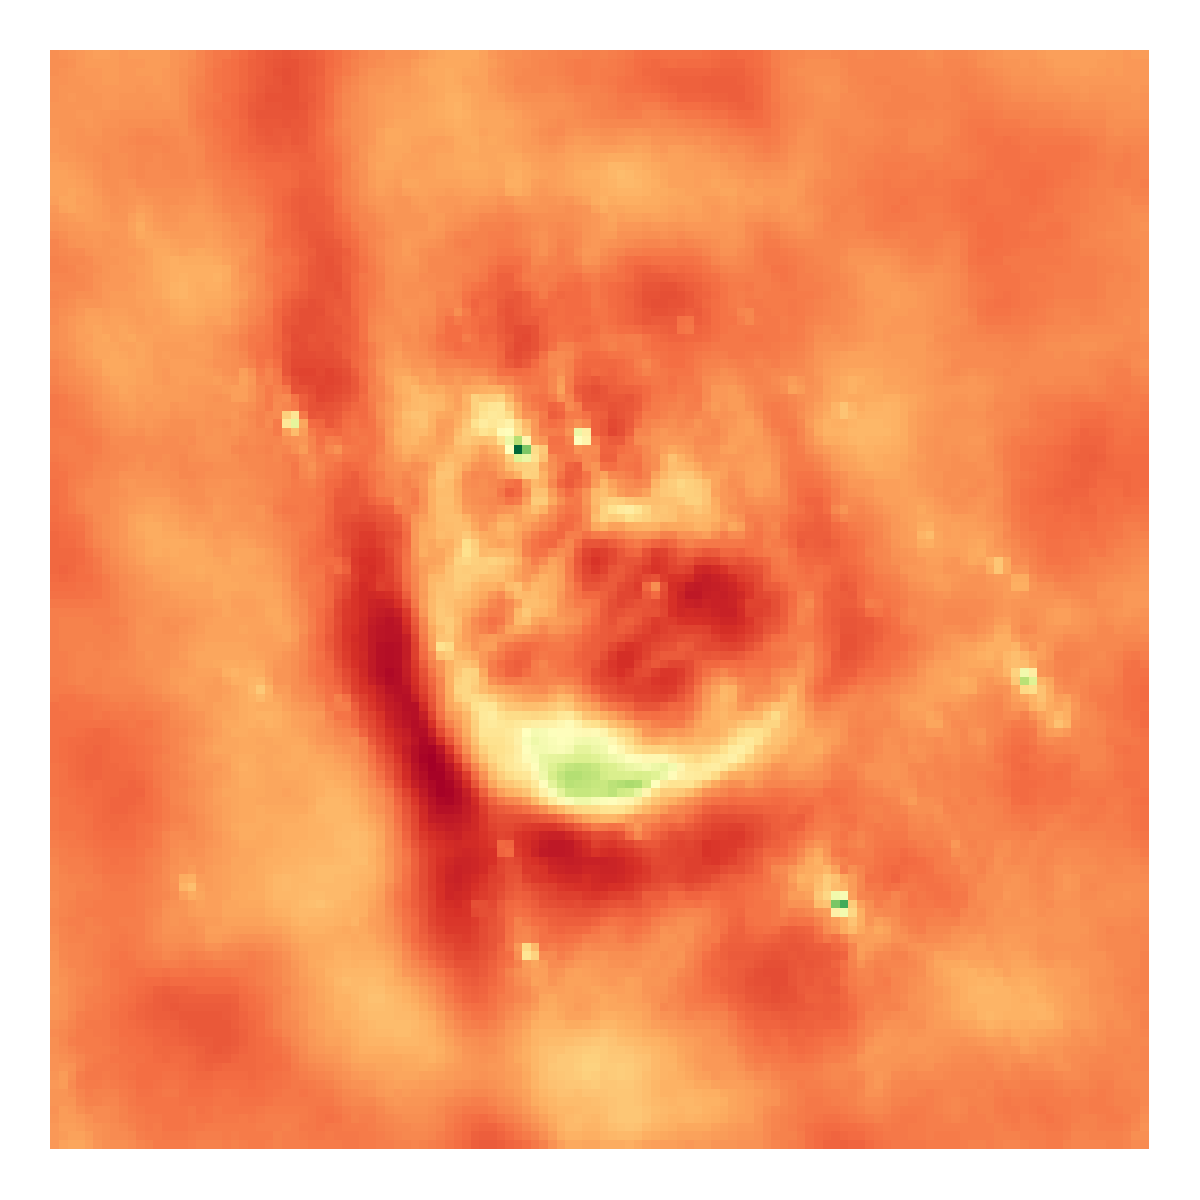
\includegraphics[width=\linewidth, trim={18px 19px 18px 18px}, clip]{./chapters/05.results/g55/raw_model.png}
	\end{subfigure}
	\begin{subfigure}[b]{0.24\linewidth}
		\centering{CLEAN}
		
\includegraphics[width=\linewidth, trim={18px 19px 18px 18px}, clip]{./chapters/05.results/g55/clean_model.png}
	\end{subfigure}
	\begin{subfigure}[b]{0.24\linewidth}
		\centering{No Regularization}
		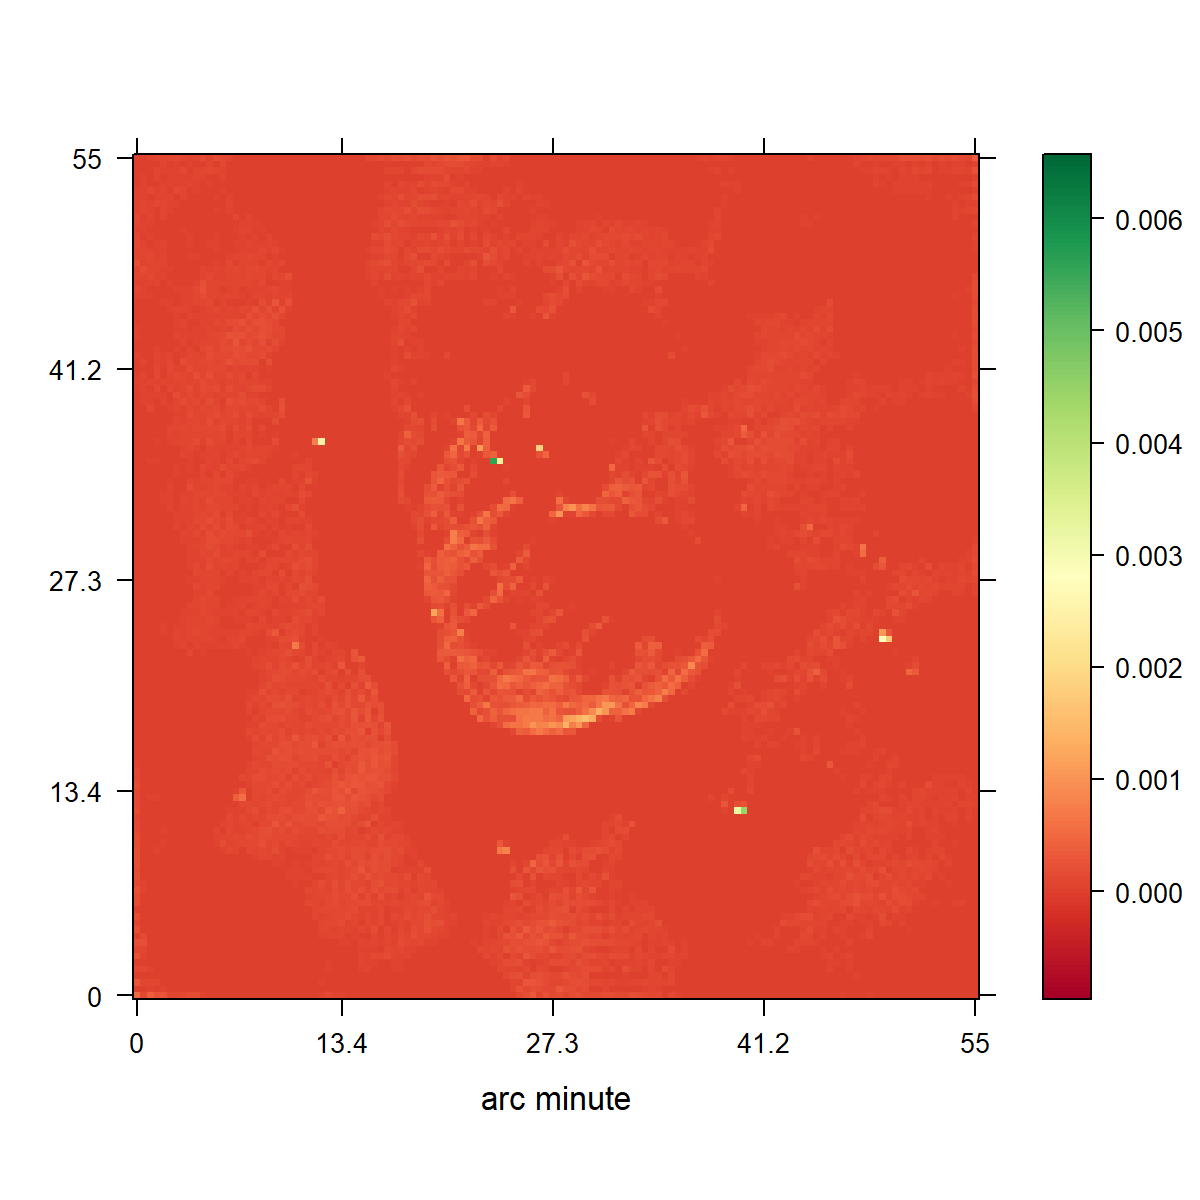
\includegraphics[width=\linewidth, trim={18px 19px 18px 18px}, clip]{./chapters/05.results/g55/positive_deconv_model.png}
	\end{subfigure}
	\begin{subfigure}[b]{0.24\linewidth}
		\centering{L1}
		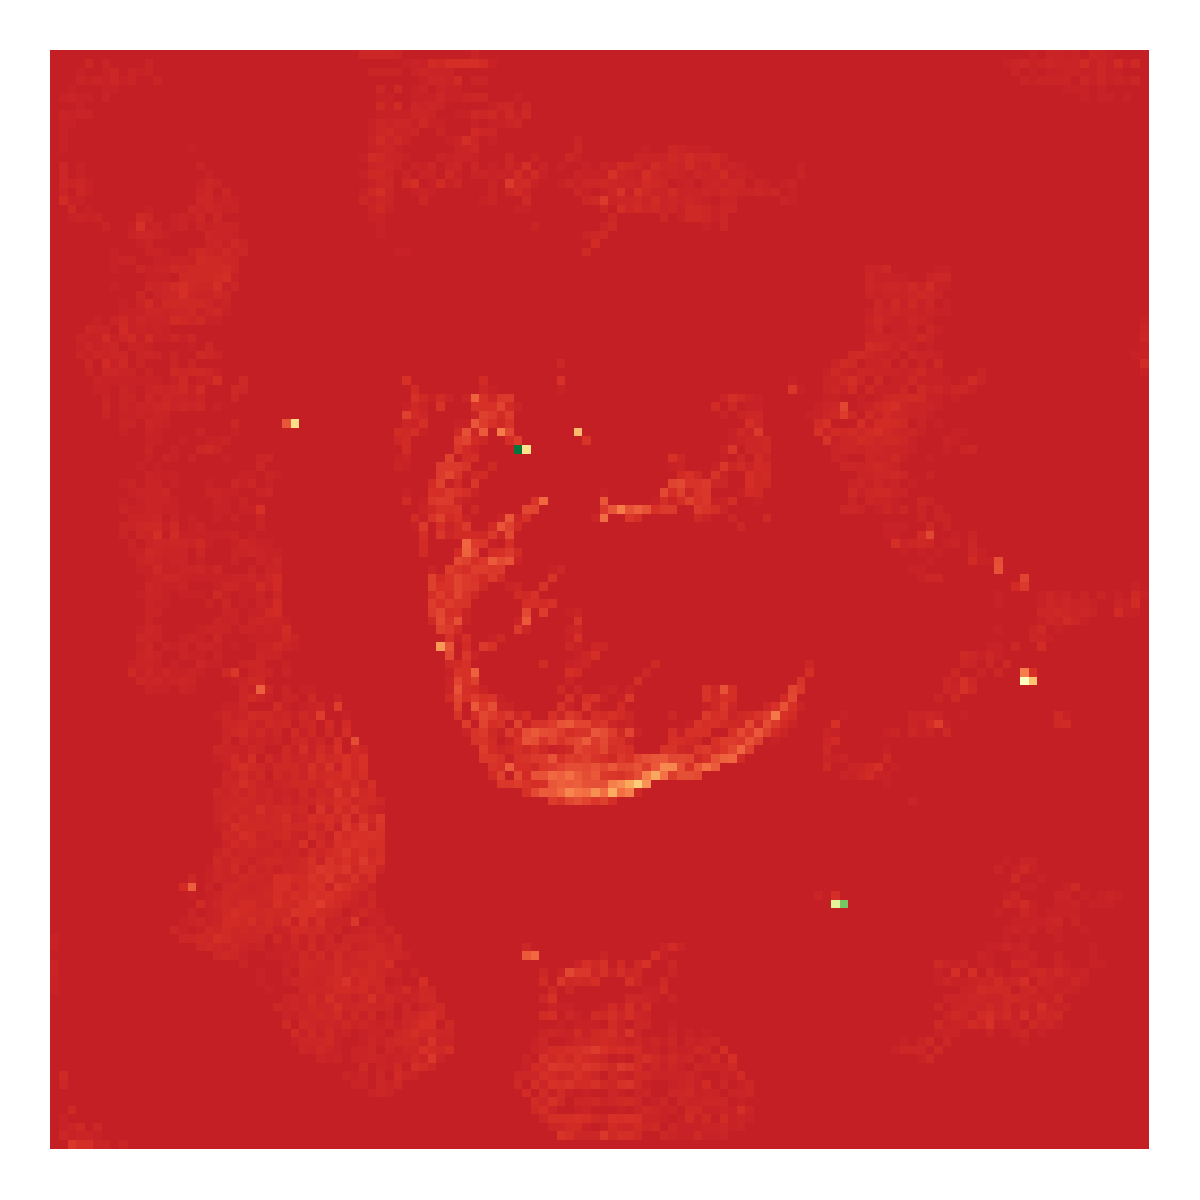
\includegraphics[width=\linewidth, trim={18px 19px 18px 18px}, clip]{./chapters/05.results/g55/L1_model.png}
	\end{subfigure}
	
	\begin{subfigure}[b]{0.24\linewidth}
		\vspace{10pt}
		\centering{L2}
		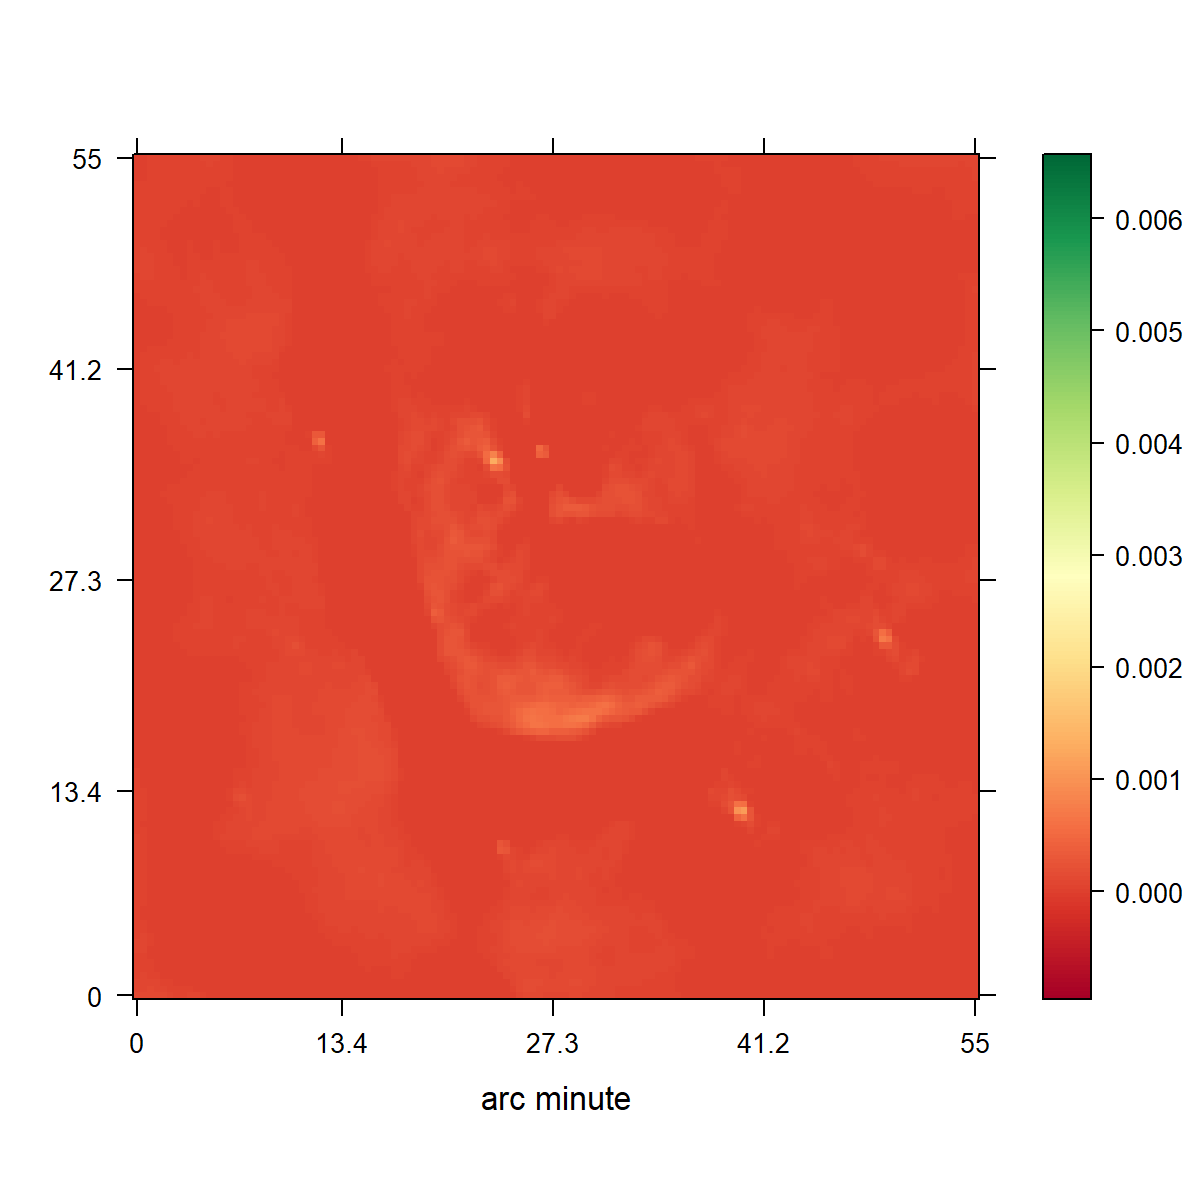
\includegraphics[width=\linewidth, trim={18px 19px 18px 18px}, clip]{./chapters/05.results/g55/L2_model.png}
	\end{subfigure}
	\begin{subfigure}[b]{0.24\linewidth}
		\centering{L1+L2}
		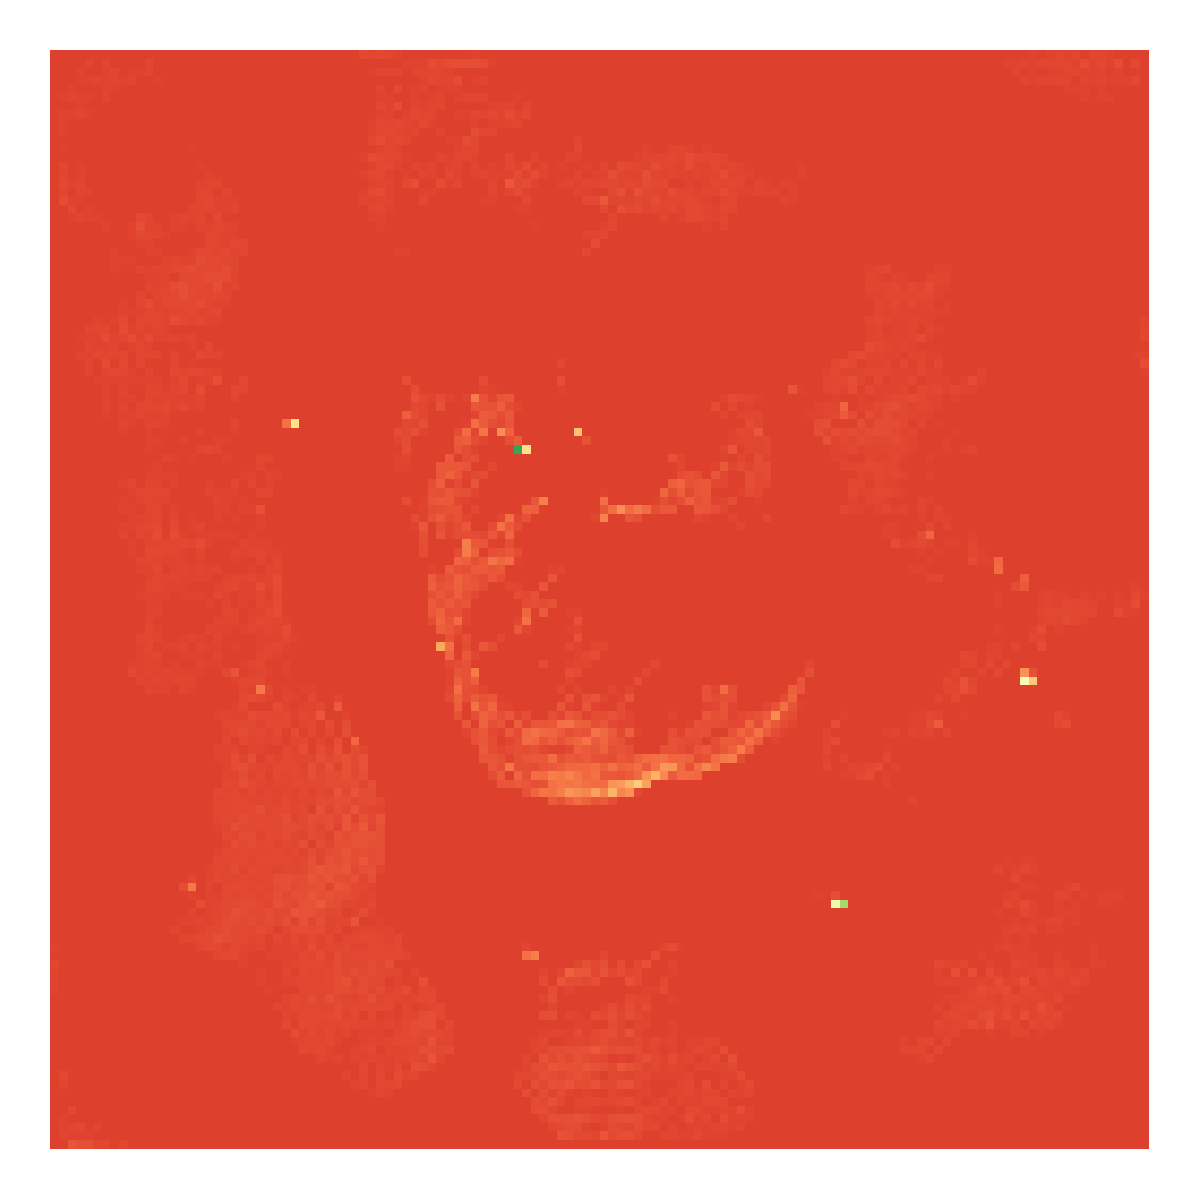
\includegraphics[width=\linewidth, trim={18px 19px 18px 18px}, clip]{./chapters/05.results/g55/L1+L2_model.png}
	\end{subfigure}
	\begin{subfigure}[b]{0.24\linewidth}
		\centering{Total Variation}
		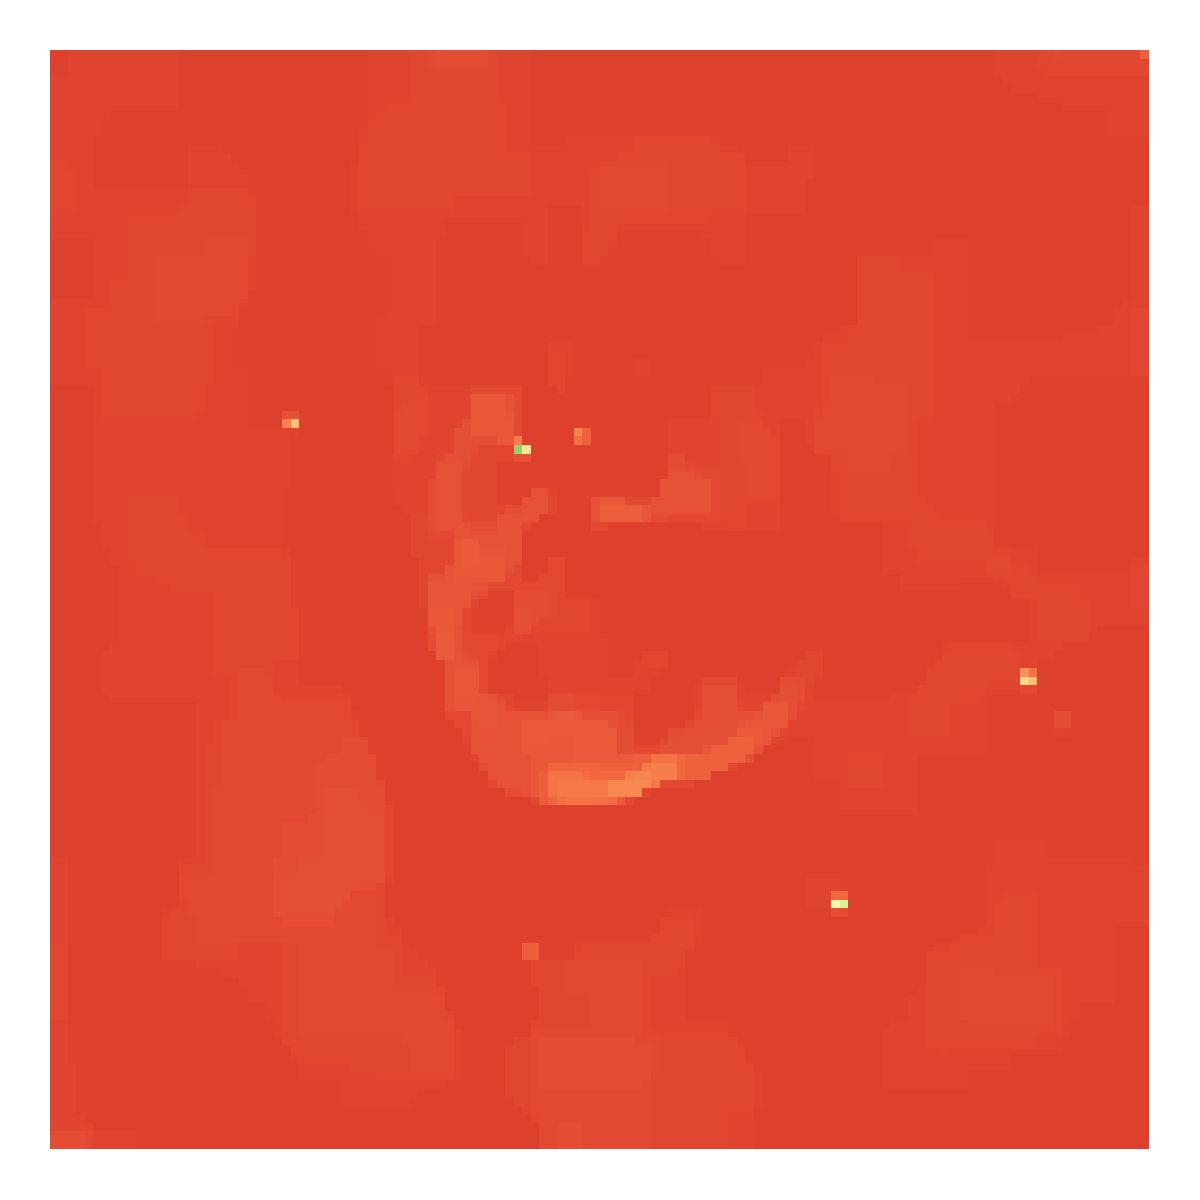
\includegraphics[width=\linewidth, trim={18px 19px 18px 18px}, clip]{./chapters/05.results/g55/TV_model.png}
	\end{subfigure}
	\begin{subfigure}[b]{0.24\linewidth}
		\centering{Starlets}
		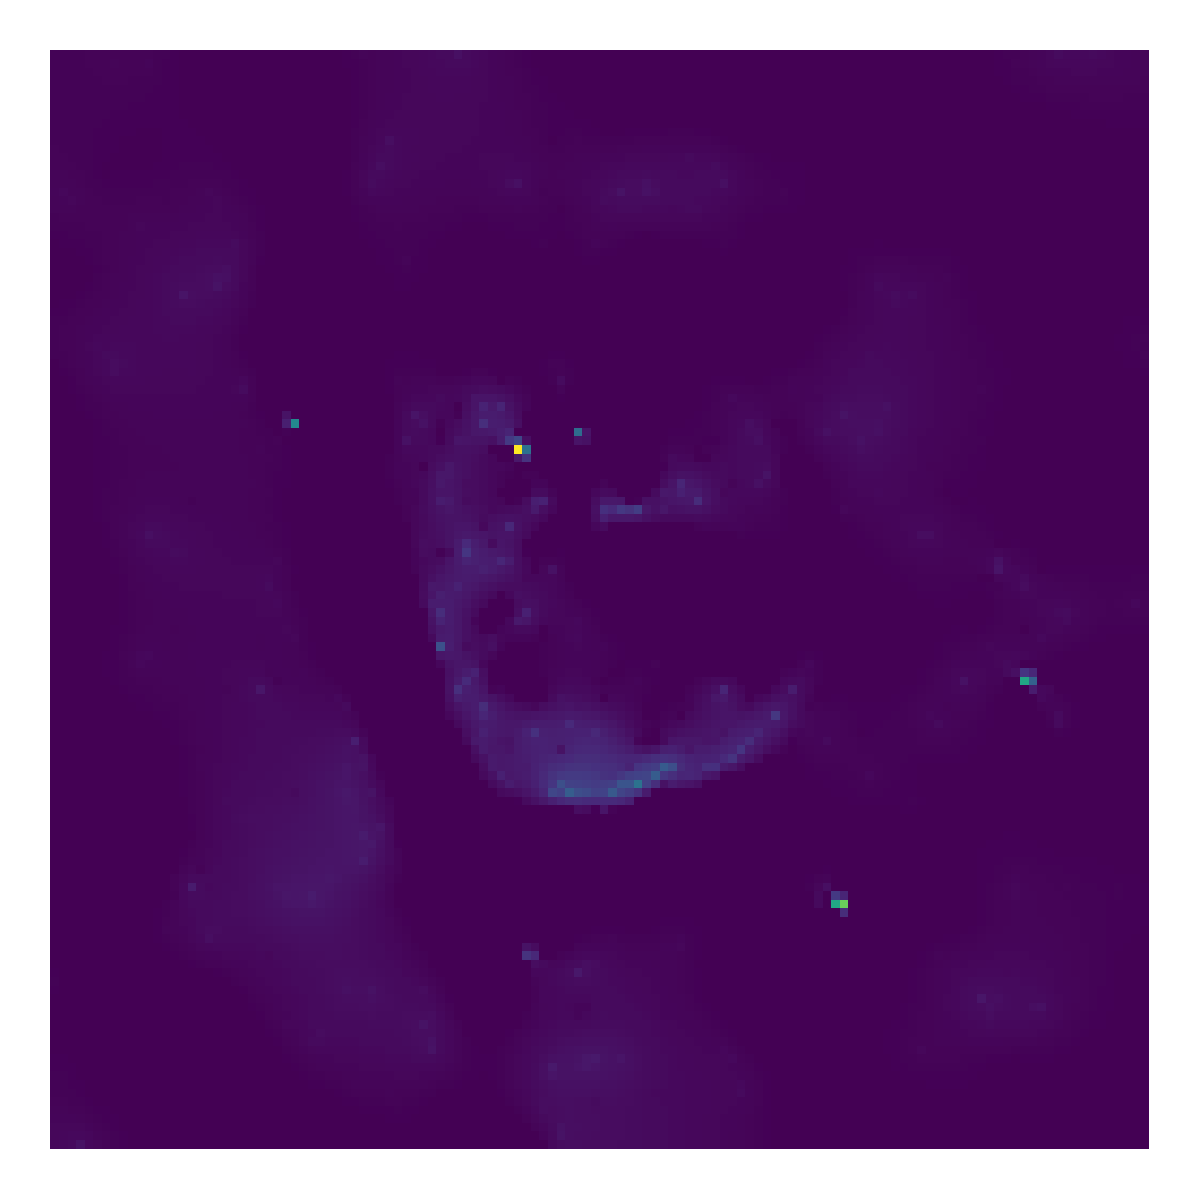
\includegraphics[width=\linewidth, trim={18px 19px 18px 18px}, clip]{./chapters/05.results/g55/starlets3_model.png}
	\end{subfigure}
	\caption{Reconstructed images of CLEAN and the different Compressed Sensing priors.} 
	\label{res:g55:img}
\end{figure}

\begin{figure}
	\centering
	\begin{subfigure}[b]{0.9\linewidth}
		\centering
		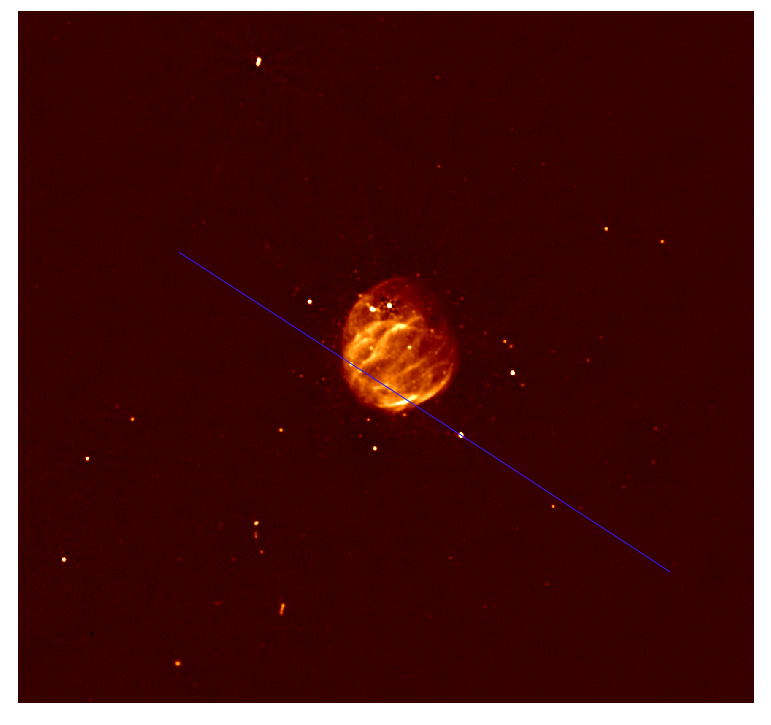
\includegraphics[width=0.3\linewidth, trim={180px 170px 170px 146px}, clip]{./chapters/05.results/pic_G55_7_lined.png}
		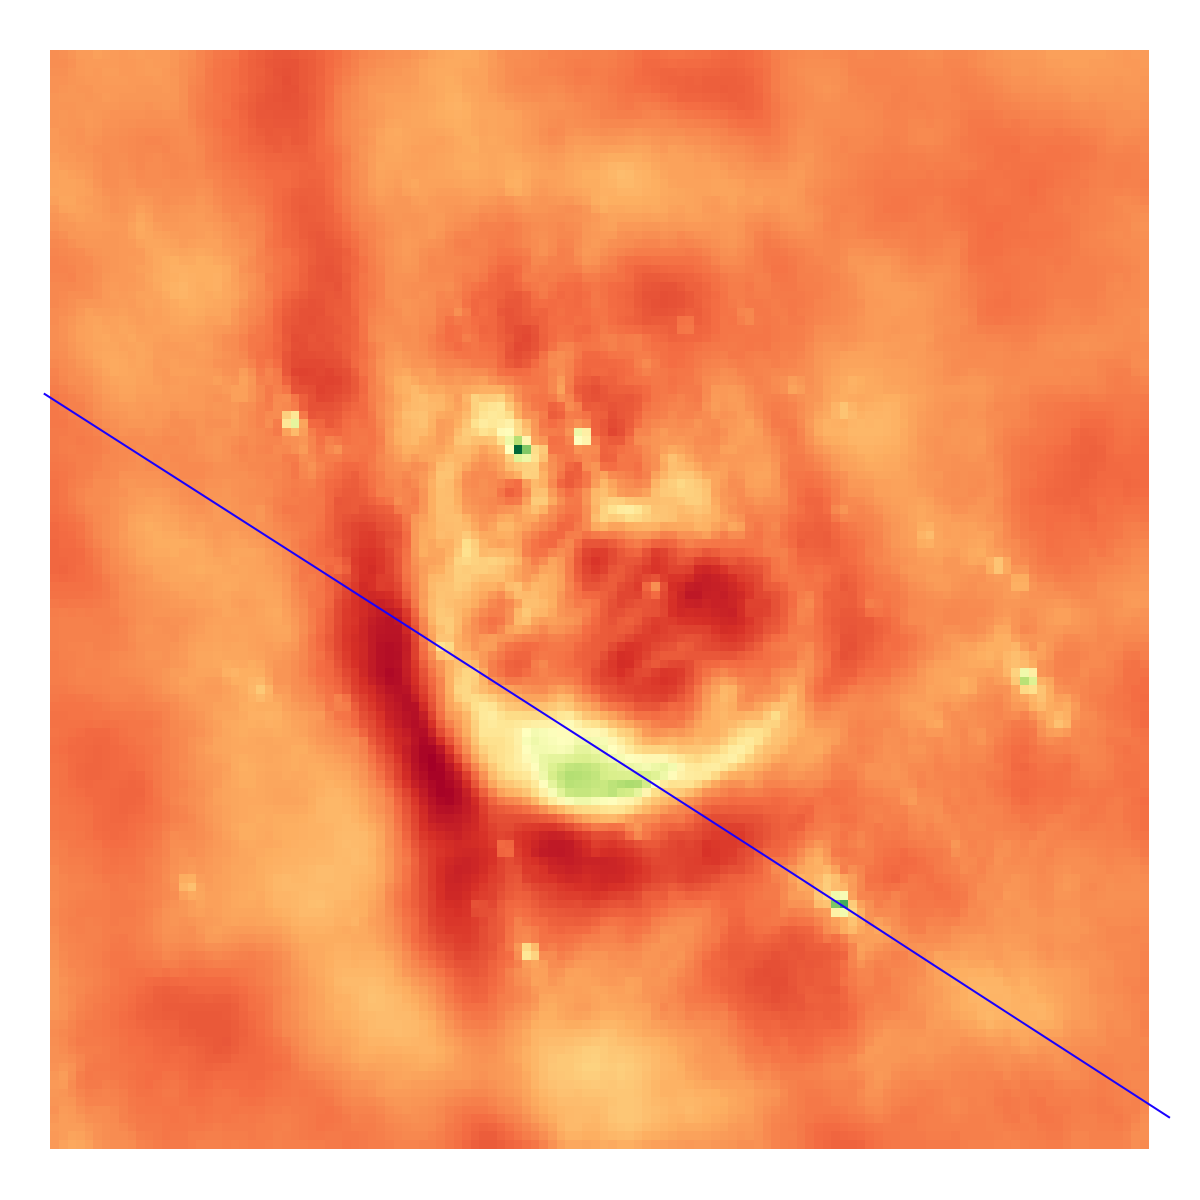
\includegraphics[width=0.3\linewidth, trim={18px 19px 18px 18px}, clip]{./chapters/05.results/raw_image_lined.png}
		\caption{profile cut}
	\end{subfigure}

	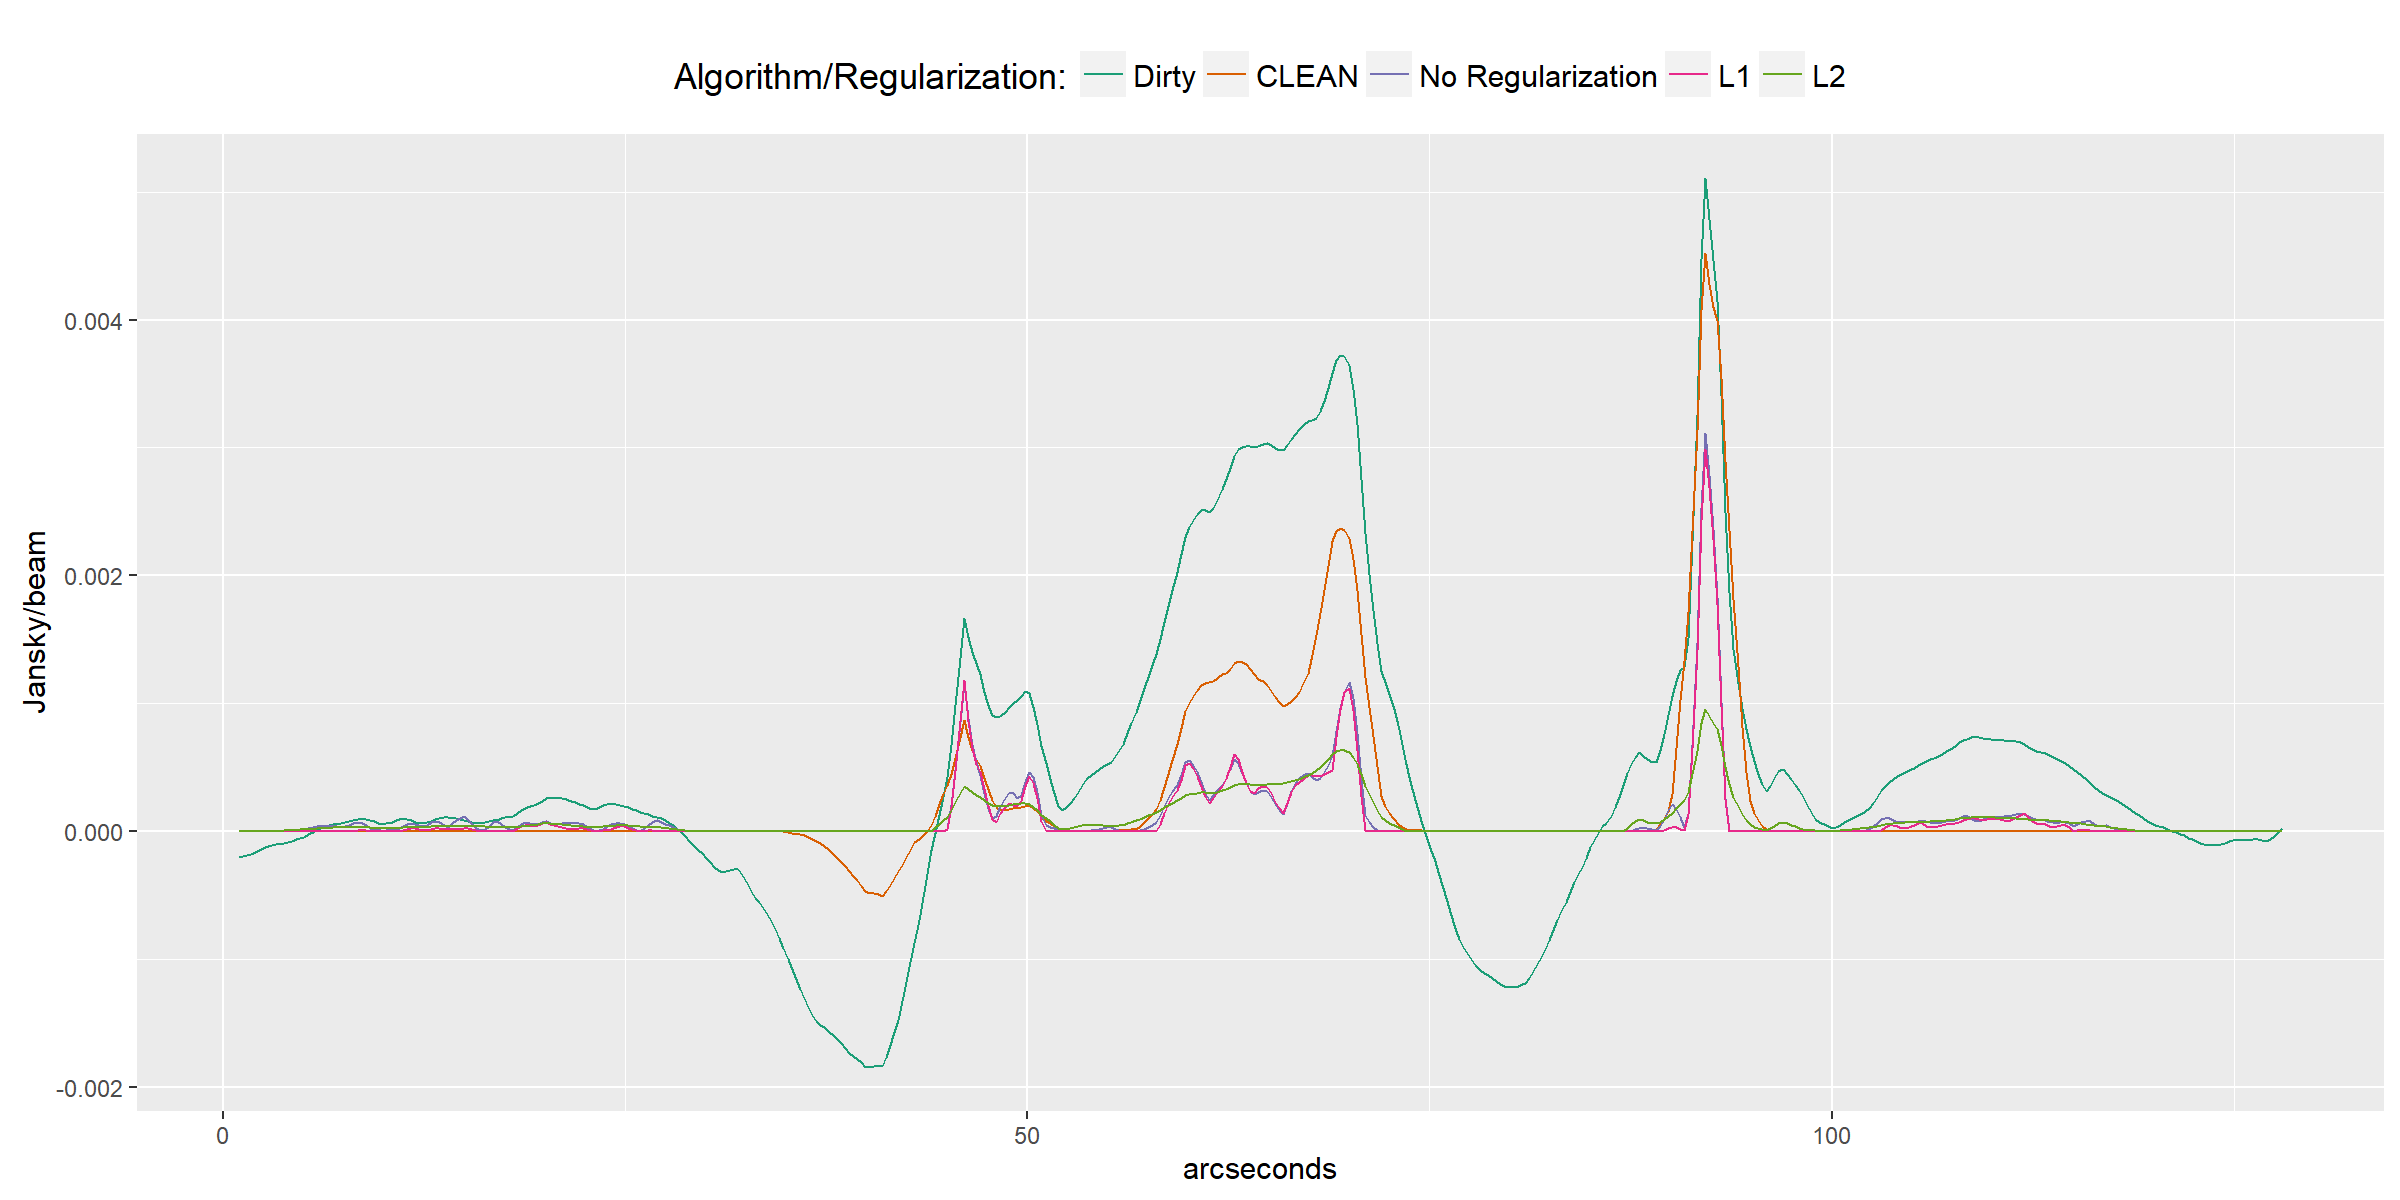
\includegraphics[width=\linewidth, clip]{./chapters/05.results/df1.png}
	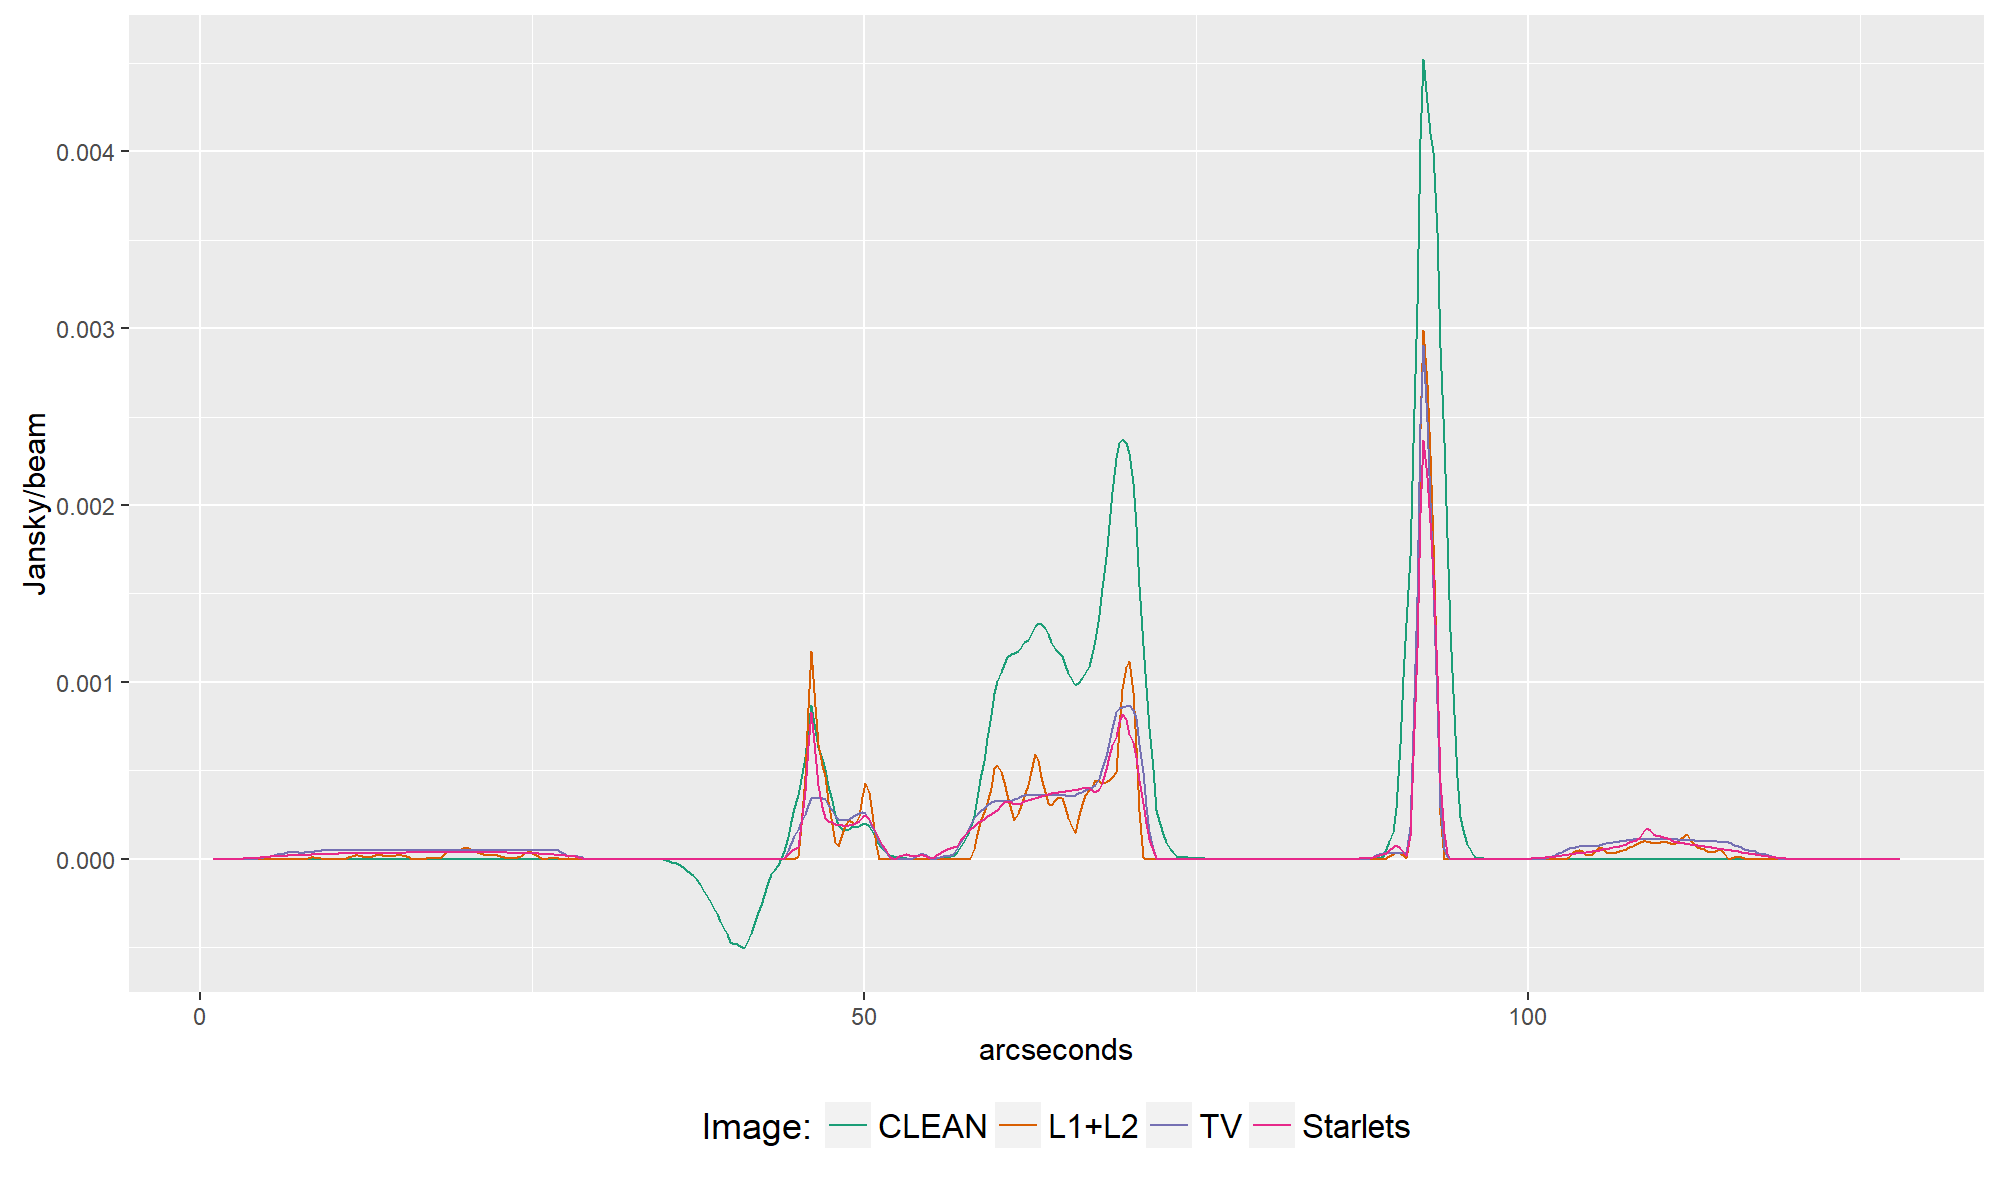
\includegraphics[width=\linewidth, clip]{./chapters/05.results/df2.png}
	\caption{Intensity profile of CLEAN and the different Compressed Sensing Regularizations.}
	\label{res:g55:profile}
\end{figure}

\textbf{CLEAN:} CLEAN detects the brightest point sources, but finds only part of the extended emission. The top half of the "egg" emission is missing. The structures of the remnant are blurred compared to the Compressed Sensing reconstructions. With the parameters of the imaging tutorial, CLEAN models the trench as a region with negative emissions. This is not physically plausible, although the behaviour can be changed with additional parameters. The profile \ref{res:g55:profile} shows that CLEAN accurately reconstructs the flux of the large peaks, although the peaks are wide in comparison.

\textbf{No Regularization:} Detects the Egghead of the remnant and the non-negativity constraint keeps it from modelling the negative trench. It detects the smaller emissions around the remnant, but also detects "fake" extended emissions. The profile \ref{res:g55:profile}  shows two smaller peaks in the center which also appear in \ref{results:g55:nrao:rec} as do the two small point sources at the edge of the remnant. However, the dirty image has a rise in flux at the borders of the image, which is likely an artefact of the measurement, considering it does not exist in the NRAO reconstruction \ref{results:g55:nrao:rec}.

\textbf{L1:} There is almost no visible difference between no regularization and L1. This is possibly an interaction with the Miller $\lambda$ estimation, since the result of no regularization was used to estimate the $\lambda$ of L1. The L1 regularization removes part of the "fake" extended emission, particularly in the top region, but also a few structures in the center. The peaks in the profile \ref{res:g55:profile} of L1 and no regularization are narrower than CLEAN, although they do not reach the same peak flux. L1 is prone to produce unlikely extended emissions: L1 also tries to approximate extended emissions with a number of faint point sources. This can introduce artefacts like pixel wide holes in extended emissions.

\textbf{L2:} Forces the extended emissions to be more smooth. It also considerably lowers the flux of bright point sources. The profile \ref{res:g55:profile} shows L2 forces the bright peak to widen and lower. The peak is almost as wide as the CLEAN reconstruction. In the remnant center, it smoothers the smaller peaks.

\textbf{L1+L2}: Since L1 does a good job with point sources, but needs to be more continuous for extended emissions, why does one not combine both regularizations? The flexibility of Compressed Sensing Reconstructions allows for it. Sadly, the result is indistinguishable from the L1 regularization. In the dirty image, all pixels are very close to zero (Maximum: 0.0076 in Dirty Image). If the L1 and L2 regularization receive the same $\lambda$, the L1 term dominates. If the dirty image would contain pixels much larger than 1, then the L2 term would dominate.

\textbf{Total Variation:} A simple prior that has its origins in image de-noising. The objective is to reduce the gradients over the image. With an infinite $\lambda$, the Total Variation forces all pixels of the reconstruction to have the same value. The idea of the prior is to work well for both extended emissions and point sources. It has trouble with point sources inside extended emissions. In the profile, it is clearly visible how Total Variations cuts the peaks inside the remnant.

\textbf{Starlets:} Is a more sophisticated prior which also tries to model both point sources and extended emissions. It locates the point sources accurately. In the profile \ref{res:g55:profile} it also finds the faint point sources in the extended emission. However, it also smoothed out the structure inside the remnant. For the LOFAR instrument, the starlet regularization was able to find smaller structures than the antenna beam-width\cite{girard2015sparse}. The smallest starlet has a $5*5$ pixels dimension. For this reconstruction, the antenna beam-width is about two pixels wide. The resolution might be too coarse for the starlet regularization.

CLEAN produces the most accurate flux for strong point sources, even though in other reports Total Variation and Starlets reconstructed comparable peak flux to CLEAN \cite{garsden2015lofar}\cite{mcewen2011compressed}.This is due to the implementation in CASA: The PSF CASA produces does not sum up to one. Convolving an image with the PSF increases the total flux, and naturally a deconvolution decreases the flux. CLEAN is the only algorithm that comes close to the measured flux, because in the last iteration, the reconstructed image gets convolved with the beam pattern (usually a 2d gaussian function), which is also not normalized. If we also convolve the Compressed Sensing reconstructions with the beam pattern (and smear away details), the fluxes become similar.

In this example, the L1 normalization was able to find smaller, plausible structures than CLEAN inside the remnant. Outside the remnant, all Compressed Sensing Reconstructions found "fake" extended emissions. The L2 and starlet were also expected to find smaller structures. One possible explanation is that the antenna beam-width is about two pixels wide. Any structure smaller than the beam-width is one pixel wide.

For higher resolutions it is expected that L1 introduces more artefacts. The current implementation cannot increase the resolution since it needs a quadratic amount of memory per pixel: The image size of about $128^2$ was the maximum which was feasible to solve on a laptop. The convolution operation $x \star PSF$ gets modelled as a matrix-vector product. The matrix therefore has $128^4$ entries.

